\documentclass[12pt]{report}

% ============================================================
% PACKAGES
% ============================================================
\usepackage{iftex}
\usepackage[a4paper,margin=1in,top=1.3in,bottom=1.3in]{geometry}
\usepackage[table]{xcolor}
\usepackage{titlesec}
\usepackage{fancyhdr}
\usepackage[hidelinks,hypertexnames=false]{hyperref}
\usepackage{amsmath,amssymb}
\usepackage{graphicx}
\usepackage{tikz}
\usetikzlibrary{arrows.meta,positioning,shapes.geometric}
\usepackage{enumitem}
\usepackage{booktabs}
\usepackage{longtable}
\usepackage{array}
\usepackage{tcolorbox}
\tcbuselibrary{skins,breakable}
\usepackage{tocloft}
\usepackage{setspace}
\usepackage{multicol}
\usepackage[nopatch=footnote]{microtype}
\usepackage{etoolbox}

% ============================================================
% FONTS
% Gilroy is used for body text and Bebas Neue for headings as specified.
% Fallbacks provided for portable compilation.
% ============================================================
\ifPDFTeX
  \usepackage[utf8]{inputenc}
  \usepackage[T1]{fontenc}
  \usepackage{lmodern}
  \newcommand{\headingfont}{\sffamily}
  \newcommand{\displayfont}{\sffamily}
  \newcommand{\monofont}{\ttfamily}
\else
  \usepackage{fontspec}
  \IfFontExistsTF{Gilroy}{
    \setmainfont{Gilroy}[
      UprightFont = Gilroy-Regular,
      BoldFont = Gilroy-Bold,
      ItalicFont = Gilroy-RegularItalic,
      BoldItalicFont = Gilroy-BoldItalic
    ]
  }{
    \IfFontExistsTF{Gilroy-Regular}{
      \setmainfont{Gilroy-Regular}[
        BoldFont = Gilroy-Bold,
        ItalicFont = Gilroy-RegularItalic,
        BoldItalicFont = Gilroy-BoldItalic
      ]
    }{
      \IfFontExistsTF{Montserrat}{
        \setmainfont{Montserrat}
      }{
        \setmainfont{Segoe UI}
      }
    }
  }
  \IfFontExistsTF{Bebas Neue}{
    \newfontfamily\headingfont{Bebas Neue}[BoldFont = *]
    \newfontfamily\displayfont{Bebas Neue}[BoldFont = *]
  }{
    \IfFontExistsTF{Impact}{
      \newfontfamily\headingfont{Impact}[BoldFont = *]
      \newfontfamily\displayfont{Impact}[BoldFont = *]
    }{
      \newfontfamily\headingfont{Arial}
      \newfontfamily\displayfont{Arial}
    }
  }
  \IfFontExistsTF{Liberation Mono}{
    \newfontfamily\monofont{Liberation Mono}
  }{
    \IfFontExistsTF{Consolas}{
      \newfontfamily\monofont{Consolas}
    }{
      \newfontfamily\monofont{Courier New}
    }
  }
\fi

% ============================================================
% HABIB UNIVERSITY / OSL BRAND PALETTE (as used in PPP MoUs)
% ============================================================
\definecolor{HUPurple}{HTML}{4B2C6F}
\definecolor{HUGold}{HTML}{C9A24B}
\definecolor{HUDark}{HTML}{1A1A1A}
\definecolor{HUGrey}{HTML}{5A5A5A}
\definecolor{HULight}{HTML}{F7F3EE}

% ============================================================
% SECTION STYLING
% ============================================================
\titleformat{\chapter}[display]
  {\displayfont\fontsize{34}{34}\selectfont\color{HUPurple}}
  {\filright\displayfont\Large\color{HUGold}CHAPTER \thechapter}
  {6pt}
  {\titlerule[1pt]\vspace{8pt}}
\titlespacing*{\chapter}{0pt}{0pt}{20pt}

\titleformat{\section}
  {\headingfont\Large\bfseries\color{HUPurple}\raggedright}
  {\thesection}{10pt}{}
\titleformat{\subsection}
  {\headingfont\large\bfseries\color{HUDark}\raggedright}
  {\thesubsection}{8pt}{}
\titleformat{\subsubsection}
  {\headingfont\normalsize\bfseries\color{HUGrey}\raggedright}
  {\thesubsubsection}{6pt}{}

% ============================================================
% HEADER / FOOTER
% ============================================================
\setlength{\headheight}{14pt}
\pagestyle{fancy}
\fancyhf{}
\renewcommand{\headrulewidth}{0.6pt}
\renewcommand{\footrulewidth}{0.4pt}
\fancyhead[L]{\headingfont\small\color{HUGrey}Rover Navigation Simulator}
\fancyhead[R]{\headingfont\small\color{HUGrey}Linear Algebra Project Guide}
\fancyfoot[C]{\headingfont\small\color{HUGrey}Habib University}
\fancyfoot[R]{\headingfont\small\color{HUGrey}\thepage}

\fancypagestyle{plain}{
  \fancyhf{}
  \fancyfoot[C]{\headingfont\small\color{HUGrey}\thepage}
  \renewcommand{\headrulewidth}{0pt}
}

% ============================================================
% TABLE OF CONTENTS STYLING
% ============================================================
\renewcommand{\cftchapfont}{\headingfont\bfseries\color{HUPurple}}
\renewcommand{\cftsecfont}{\headingfont\color{HUDark}}
\renewcommand{\cftchappagefont}{\headingfont\color{HUPurple}}
\renewcommand{\cftsecpagefont}{\headingfont\color{HUDark}}

% ============================================================
% CUSTOM ENVIRONMENTS
% ============================================================
\newtcolorbox{infobox}[1][]{
  breakable, enhanced, colback=HULight, colframe=HUPurple,
  boxrule=0.8pt, arc=2pt, left=8pt, right=8pt, top=6pt, bottom=6pt,
  fonttitle=\headingfont\bfseries, coltitle=white,
  colbacktitle=HUPurple, fontupper=\raggedright, #1
}

\newtcolorbox{phasebox}[1]{
  breakable, enhanced, colback=white, colframe=HUGold,
  boxrule=1pt, arc=2pt, left=8pt, right=8pt, top=6pt, bottom=6pt,
  fonttitle=\headingfont\bfseries\large, coltitle=white,
  colbacktitle=HUPurple, fontupper=\raggedright, title=#1
}

\newtcolorbox{pseudobox}[1]{
  breakable, enhanced, colback=HUDark!3, colframe=HUDark,
  boxrule=0.6pt, arc=1pt, left=8pt, right=8pt, top=6pt, bottom=6pt,
  fonttitle=\monofont\bfseries, coltitle=white,
  colbacktitle=HUDark, fontupper=\small, title=#1
}

\BeforeBeginEnvironment{verbatim}{\small}

\newcommand{\qanda}[2]{
  \par\vspace{4pt}\noindent\headingfont\bfseries\color{HUPurple}Q: \normalfont\color{HUDark}#1\par
  \noindent\headingfont\bfseries\color{HUGold}A: \normalfont\color{black}#2\par\vspace{2pt}
}

\setlist[itemize]{label=\textcolor{HUPurple}{\textbullet}}
\newlist{checklist}{itemize}{1}
\setlist[checklist]{label=$\square$, leftmargin=*}

% ============================================================
% DOCUMENT
% ============================================================
\begin{document}

% ---------------- TITLE PAGE ----------------
\begin{titlepage}
\centering
\vspace*{0.4cm}
{\headingfont\color{HUGrey}\large HABIB UNIVERSITY\par}
{\headingfont\color{HUGrey}\normalsize Dhanani School of Science and Engineering\par}
\vspace{0.3cm}
{\color{HUGold}\rule{0.6\linewidth}{1.2pt}\par}
\vspace{1.8cm}

{\displayfont\color{HUPurple}\fontsize{52}{52}\selectfont ROVER NAVIGATION\par}
{\displayfont\color{HUPurple}\fontsize{52}{52}\selectfont SIMULATOR\par}
\vspace{0.4cm}
{\headingfont\color{HUDark}\Large Linear Algebra Project --- Development and Preparation Guide\par}

\vspace{1.6cm}
{\color{HUGold}\rule{0.35\linewidth}{0.8pt}\par}
\vspace{1.6cm}

\begin{tabular}{ll}
\headingfont\bfseries\color{HUPurple}Course: & \color{HUDark}Linear Algebra \\[4pt]
\headingfont\bfseries\color{HUPurple}Author: & \color{HUDark}Sheikh Muhammad Muneeb \\[4pt]
\headingfont\bfseries\color{HUPurple}Group Members: & \color{HUDark}Sheikh M Muneeb \\
 & \color{HUDark}Misha Jessani \\
 & \color{HUDark}Adil Saleem \\[4pt]
\headingfont\bfseries\color{HUPurple}Instructor: & \color{HUDark}Rameez Raghib \\[4pt]
\headingfont\bfseries\color{HUPurple}Submission Date: & \color{HUDark}30th July, 2026 \\
\end{tabular}

\vfill
{\headingfont\color{HUGrey}\small Karachi, Pakistan\par}
\end{titlepage}

% ---------------- TOC ----------------
\pagenumbering{roman}
\tableofcontents
\clearpage
\pagenumbering{arabic}

% ============================================================
\chapter{Project Introduction}
% ============================================================

\section{What is the Rover Navigation Simulator}
The Rover Navigation Simulator models a planetary rover in an unknown terrain. The rover receives a sequence of movement commands (translate, rotate, or a combination of both) and the simulator computes the rover's resulting position and orientation after each command using linear algebra, specifically transformation matrices. The simulator tracks and visualizes the complete trajectory of the rover from its starting configuration to its final state.

\section{Why Linear Algebra Matters Here}
\begin{infobox}[title=Core Idea]
Every movement of a rigid body in 2D or 3D space, whether a translation, a rotation, or a combination of the two, can be represented and computed using vectors and matrices. This project exists specifically to make that abstraction concrete.
\end{infobox}

\begin{itemize}
\item \textbf{Vectors} encode the rover's position and heading as numerical quantities that can be manipulated algebraically.
\item \textbf{Matrices} encode linear transformations (rotation, translation) as operators acting on those vectors.
\item \textbf{Matrix multiplication} allows multiple transformations to be composed into a single operation, which is essential when a rover executes a long sequence of commands.
\item \textbf{Homogeneous coordinates} allow rotation and translation, which are mathematically different types of operations, to be unified into a single matrix multiplication.
\end{itemize}

\section{Real-World Applications}
\begin{itemize}
\item \textbf{Planetary exploration:} Rovers such as NASA's Perseverance and Curiosity use transformation-matrix-based localization to track position on Mars.
\item \textbf{Robotics:} Mobile robots and robotic arms rely on transformation chains to compute end-effector or chassis position relative to a base frame.
\item \textbf{Autonomous navigation:} Self-driving vehicles use coordinate transformations to convert sensor data between local and global reference frames.
\item \textbf{Computer graphics:} Game engines and rendering pipelines apply rotation, translation, and homogeneous coordinate machinery to orient objects in a 3D scene.
\end{itemize}

% ============================================================
\chapter{Project Objectives}
% ============================================================

\section{Technical Objectives}
\begin{checklist}
\item Design and implement a rover state representation (position and orientation).
\item Implement a command parser capable of interpreting movement instructions.
\item Build a matrix operations engine supporting translation and rotation.
\item Implement transformation chaining across an arbitrary sequence of commands.
\item Store and visualize the rover's complete trajectory.
\item Support a fully configurable starting pose and target end point at runtime, so the rover's mission is never hardcoded.
\item Derive the trajectory connecting a start and end point automatically from displacement geometry, rather than requiring a hand-scripted command sequence.
\item Produce a complete, human-readable matrix calculation trace for every transformation applied, suitable for direct instructor review.
\item Validate correctness through structured test cases.
\end{checklist}

\section{Mathematical Objectives}
\begin{checklist}
\item Demonstrate correct construction of 2D (and optionally 3D) rotation matrices.
\item Demonstrate correct construction of translation vectors and matrices.
\item Demonstrate proper use of homogeneous coordinates to unify translation and rotation.
\item Demonstrate correct order-dependent matrix multiplication for chained transformations.
\item Verify numerical accuracy of trajectories against hand calculations.
\end{checklist}

% ============================================================
\chapter{Mathematical Foundation}
% ============================================================

\section{Vectors and Rover State Representation}
The rover's state at any time step can be represented as a vector describing its position and heading:
\begin{equation}
\mathbf{s} = \begin{bmatrix} x \\ y \\ \theta \end{bmatrix}
\end{equation}
where $x,y$ denote the rover's position in the 2D plane and $\theta$ denotes its heading angle relative to a fixed reference axis.

\section{Coordinate Systems}
The simulator distinguishes between two frames of reference:
\begin{itemize}
\item \textbf{World frame:} A fixed global coordinate system in which the rover's absolute position is expressed.
\item \textbf{Rover (local) frame:} A coordinate system attached to the rover itself, in which movement commands such as ``move forward'' are naturally expressed.
\end{itemize}
Every movement command issued in the rover's local frame must be transformed into the world frame before the rover's global state is updated.

\section{Translation Vectors}
A pure translation shifts the rover's position without changing its heading:
\begin{equation}
\mathbf{p}' = \mathbf{p} + \mathbf{t}, \qquad
\mathbf{t} = \begin{bmatrix} t_x \\ t_y \end{bmatrix}
\end{equation}

\section{Rotation Matrices in 2D}
A rotation by angle $\theta$ about the origin is given by:
\begin{equation}
R(\theta) =
\begin{bmatrix}
\cos\theta & -\sin\theta \\
\sin\theta & \cos\theta
\end{bmatrix}
\end{equation}
Applying this matrix to a position vector $\mathbf{p} = [x\ \ y]^T$ produces the rotated vector $\mathbf{p}' = R(\theta)\,\mathbf{p}$.

\subsection{Optional: Rotation Matrices in 3D}
If the rover's motion is extended to three dimensions, rotation about the individual coordinate axes is given by:
\begin{equation}
R_z(\theta) =
\begin{bmatrix}
\cos\theta & -\sin\theta & 0 \\
\sin\theta & \cos\theta & 0 \\
0 & 0 & 1
\end{bmatrix}
\end{equation}
with analogous matrices $R_x(\theta)$ and $R_y(\theta)$ for rotation about the $x$ and $y$ axes respectively.

\section{Homogeneous Coordinates}
Rotation is a linear operation, but translation is not; it cannot be expressed as a matrix multiplication in ordinary 2D or 3D coordinates. Homogeneous coordinates resolve this by appending an extra coordinate equal to 1:
\begin{equation}
\mathbf{p}_h = \begin{bmatrix} x \\ y \\ 1 \end{bmatrix}
\end{equation}
This allows both rotation and translation to be applied through a single matrix multiplication.

\section{Transformation Matrices}
The combined rotation-translation transformation matrix in homogeneous form is:
\begin{equation}
T(\theta, t_x, t_y) =
\begin{bmatrix}
\cos\theta & -\sin\theta & t_x \\
\sin\theta & \cos\theta & t_y \\
0 & 0 & 1
\end{bmatrix}
\end{equation}
Applying this to a homogeneous position vector produces the rover's new position and orientation in a single step:
\begin{equation}
\mathbf{p}_h' = T(\theta, t_x, t_y)\, \mathbf{p}_h
\end{equation}

\section{Matrix Multiplication and Transformation Chaining}
Each command is expressed as a transformation matrix in the rover's \emph{local} frame at the moment it is issued (Section~3.2). When the rover executes a sequence of $n$ commands starting from an initial world transform $W_0$, the overall world transform after all $n$ commands is built by right-multiplying each local transform onto the accumulated result, in chronological order:
\begin{equation}
W_n = W_0 \cdot T_1 \cdot T_2 \cdots T_n
\end{equation}
Because each $T_i$ is defined relative to the rover's frame at step $i$, right-multiplication (rather than left-multiplication) correctly folds a local instruction into the accumulated world-frame pose. This single composite matrix is mathematically guaranteed to yield the same final position and heading as applying each $T_i$ step by step, since matrix multiplication is associative.
\begin{infobox}[title=Critical Detail]
Matrix multiplication is not commutative: $T_1 \cdot T_2 \neq T_2 \cdot T_1$ in general. The order in which transformations are chained directly affects the rover's final position and heading. This is one of the most common sources of implementation error in this project.
\end{infobox}

\section{Configurable Initial World Transform}
$W_0$ is not fixed at the identity matrix. It is built directly from a user-supplied starting pose $(x_0, y_0, \theta_0)$:
\begin{equation}
W_0 = T(\theta_0, x_0, y_0)
\end{equation}
using the combined transformation matrix from Section~3.7. This is what makes the rover's final resting position and heading fully manually configurable rather than hardcoded: changing $(x_0,y_0,\theta_0)$ or command sequence changes every subsequent $W_i$, and therefore the end point, without altering any code.

\section{Deriving a Route Between Two Points}
Given only a start pose $(x_0, y_0, \theta_0)$ and a target end point $(x_1, y_1)$, the simplest command sequence this rover's model can express is a single rotation followed by a single forward translation: turn to face the target, then drive straight to it. This section derives that sequence directly from the displacement geometry.

The displacement vector from start to end is:
\begin{equation}
\Delta x = x_1 - x_0, \qquad \Delta y = y_1 - y_0
\end{equation}
The straight-line distance to the target follows from the Pythagorean theorem:
\begin{equation}
d = \sqrt{\Delta x^2 + \Delta y^2}
\end{equation}
The heading required to face the target is derived via $\operatorname{atan2}(\Delta y, \Delta x)$, which works in all quadrants unlike $\arctan(\Delta y/\Delta x)$:
\begin{equation}
\theta_{\text{target}} = \operatorname{atan2}(\Delta y, \Delta x)
\end{equation}
The rotation the rover must execute before driving is the difference between this required heading and its current heading, normalized to a signed angle in $[-180^\circ, 180^\circ)$ so it always represents the shorter turn:
\begin{equation}
\Delta\theta_{\text{initial}} = \operatorname{norm}(\theta_{\text{target}} - \theta_0)
\end{equation}
If a specific final heading $\theta_1$ is also requested, a second rotation is appended after the drive:
\begin{equation}
\Delta\theta_{\text{final}} = \operatorname{norm}(\theta_1 - \theta_{\text{target}})
\end{equation}
\begin{infobox}[title={Why Rotate-Then-Drive, Not a Curved Path}]
This rover's command set only supports pure rotation and pure straight-line translation (Sections~3.4 and~3.3); it has no primitive for moving along a curve. Rotate-then-drive is therefore the minimal-command path connecting any two poses this model can express, analogous to the straight-line segments of a simplified Dubins path.
\end{infobox}

% ============================================================
\chapter{Proposed System Architecture}
% ============================================================

\section{Pipeline Overview}
\begin{center}
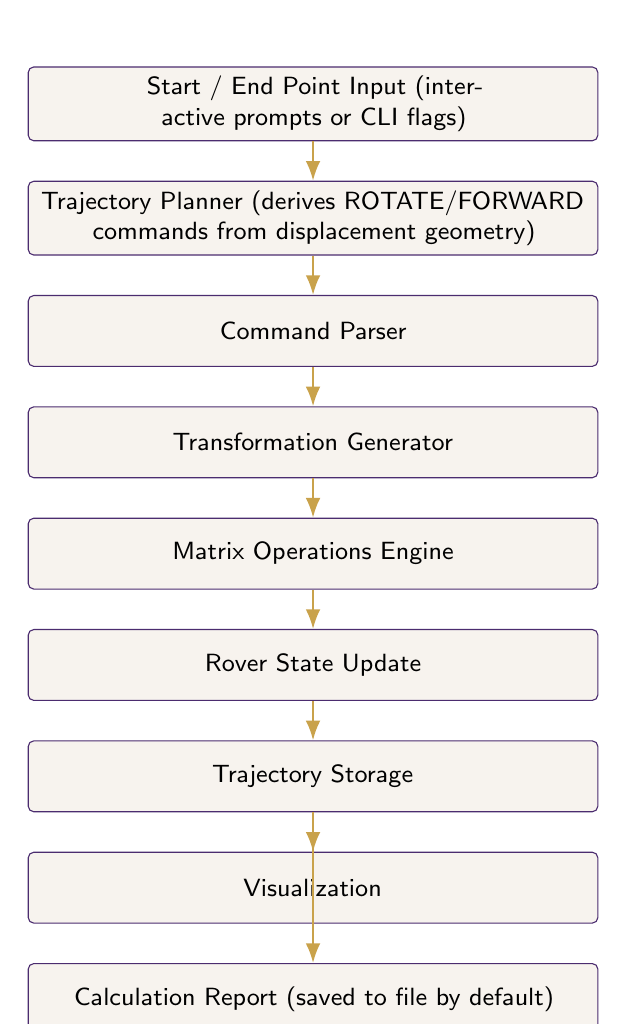
\begin{tikzpicture}[
  node distance=0.5cm,
  block/.style={rectangle, draw=HUPurple, fill=HULight, rounded corners=2pt,
    text width=7cm, align=center, minimum height=0.9cm, font=\headingfont\small},
  arrow/.style={-{Latex[length=2.5mm]}, HUGold, thick}
]
\node (n0) [block] {Start / End Point Input (interactive prompts or CLI flags)};
\node (n0b) [block, below=of n0] {Trajectory Planner (derives ROTATE/FORWARD commands from displacement geometry)};
\node (n1) [block, below=of n0b] {Command Parser};
\node (n2) [block, below=of n1] {Transformation Generator};
\node (n3) [block, below=of n2] {Matrix Operations Engine};
\node (n4) [block, below=of n3] {Rover State Update};
\node (n5) [block, below=of n4] {Trajectory Storage};
\node (n6) [block, below=of n5] {Visualization};
\node (n7) [block, below=of n6] {Calculation Report (saved to file by default)};

\draw[arrow] (n0) -- (n0b);
\draw[arrow] (n0b) -- (n1);
\draw[arrow] (n1) -- (n2);
\draw[arrow] (n2) -- (n3);
\draw[arrow] (n3) -- (n4);
\draw[arrow] (n4) -- (n5);
\draw[arrow] (n5) -- (n6);
\draw[arrow] (n5) -- (n7);
\end{tikzpicture}
\end{center}
\begin{infobox}[title=Two Input Modes]
The Command Parser accepts commands from either source: the Trajectory Planner (default point-to-point mode, shown above) or a directly supplied command sequence (legacy explicit mode, via \texttt{--commands}/\texttt{--commands-file}), which bypasses the Trajectory Planner entirely.
\end{infobox}

\section{Component Descriptions}
\begin{itemize}
\item \textbf{Start / End Point Input:} The rover's starting pose $(x_0, y_0, \theta_0)$ and target end point $(x_1, y_1, \theta_1)$, collected via interactive console prompts (the default) or CLI flags (\texttt{--start-x}/\texttt{--end-x}, etc.). Nothing about the mission or its resulting end point is hardcoded.
\item \textbf{Trajectory Planner:} Computes the minimal rotate-drive command sequence from displacement geometry (Section~3.10).
\item \textbf{Command Parser:} Converts raw command strings into typed instructions consumed by the pipeline (planner or explicit mode).
\item \textbf{Transformation Generator:} Converts each structured command into the corresponding transformation matrix (rotation, translation, or both).
\item \textbf{Matrix Operations Engine:} Performs matrix multiplication, composes chained transformations, and applies them to the rover's homogeneous position vector. Every matrix built and multiplication performed is retained as a calculation record for step-by-step arithmetic review.
\item \textbf{Rover State Update:} Updates the rover's stored position and heading based on the output of the matrix operations engine.
\item \textbf{Trajectory Storage:} Appends each new state to a running history so the full path can be reconstructed later.
\item \textbf{Visualization:} Renders the stored trajectory as a 2D (or 3D) plot showing the rover's path and orientation over time.
\item \textbf{Calculation Report:} Formats retained calculation records into a step-by-step numeric report (local matrix formulas, dot products, state extraction formulas), saved by default to \texttt{matrix\_operations.txt} for instructor review.
\end{itemize}

% ============================================================
\chapter{Step-by-Step Development Plan}
% ============================================================

\begin{phasebox}{Phase 1: Project Setup and Technology Selection}
\textbf{Goal:} Establish the development environment and finalize the technology stack. \\
\textbf{Mathematical concepts:} None (planning phase). \\
\textbf{Programming tasks:} Initialize repository; install chosen libraries; set up plotting environment; define project folder structure. \\
\textbf{Expected output:} A working, empty project skeleton that compiles/runs and can render a blank plot. \\
\textbf{Common mistakes:} Choosing a visualization library before confirming it supports the required 2D/3D plotting; not setting up version control from the start.
\end{phasebox}

\begin{phasebox}{Phase 2: Implement Vector Representation}
\textbf{Goal:} Represent the rover's state as a vector and implement basic vector operations. \\
\textbf{Mathematical concepts:} Vectors, vector addition, position representation. \\
\textbf{Programming tasks:} Define a rover state class/struct holding $x$, $y$, $\theta$; implement getters/setters; implement a print/debug method. \\
\textbf{Expected output:} A rover object that can be instantiated with an initial state and printed. \\
\textbf{Common mistakes:} Storing angle in degrees in one part of the code and radians in another without conversion.
\end{phasebox}

\begin{phasebox}{Phase 3: Implement Movement and Translation}
\textbf{Goal:} Apply pure translation to update rover position. \\
\textbf{Mathematical concepts:} Translation vectors, vector addition. \\
\textbf{Programming tasks:} Implement a \texttt{translate(tx, ty)} function; ensure translation is applied in the correct frame (local vs. world). \\
\textbf{Expected output:} Rover position updates correctly for forward, backward, or lateral movement commands. \\
\textbf{Common mistakes:} Applying translation in the world frame when the command was meant to be relative to the rover's current heading.
\end{phasebox}

\begin{phasebox}{Phase 4: Implement Rotation Matrices}
\textbf{Goal:} Apply rotation to update rover heading. \\
\textbf{Mathematical concepts:} 2D rotation matrices, trigonometric functions. \\
\textbf{Programming tasks:} Implement a \texttt{rotate(theta)} function constructing $R(\theta)$ and applying it to the heading/position as required. \\
\textbf{Expected output:} Rover heading updates correctly; test with $90^\circ$, $180^\circ$, $270^\circ$ rotations. \\
\textbf{Common mistakes:} Mixing degrees and radians when calling \texttt{sin}/\texttt{cos}; sign errors producing rotation in the wrong direction.
\end{phasebox}

\begin{phasebox}{Phase 5: Implement Homogeneous Transformations}
\textbf{Goal:} Unify rotation and translation into a single homogeneous transformation matrix. \\
\textbf{Mathematical concepts:} Homogeneous coordinates, combined transformation matrices. \\
\textbf{Programming tasks:} Implement a function that builds $T(\theta, t_x, t_y)$; convert rover position to homogeneous form before multiplication. \\
\textbf{Expected output:} A single matrix-vector multiplication correctly reproduces the combined effect of Phase 3 and Phase 4. \\
\textbf{Common mistakes:} Forgetting to append/strip the homogeneous coordinate consistently.
\end{phasebox}

\begin{phasebox}{Phase 6: Implement Transformation Chaining}
\textbf{Goal:} Support execution of an arbitrary sequence of commands via matrix composition. \\
\textbf{Mathematical concepts:} Matrix multiplication, non-commutativity, associativity. \\
\textbf{Programming tasks:} Implement a loop or reduction that multiplies transformation matrices in the correct order; apply the resulting composite matrix to the initial state. \\
\textbf{Expected output:} A sequence of five or more commands produces a final state matching manual calculation. \\
\textbf{Common mistakes:} Multiplying matrices in reverse order; not resetting the accumulator matrix between simulation runs.
\end{phasebox}

\begin{phasebox}{Phase 7: Create Trajectory Visualization}
\textbf{Goal:} Visualize the rover's full path and orientation history. \\
\textbf{Mathematical concepts:} Coordinate plotting, vector fields (for heading arrows). \\
\textbf{Programming tasks:} Store each intermediate state; plot $x$ vs. $y$ as a path; overlay heading arrows at each step. \\
\textbf{Expected output:} A 2D plot showing the rover's trajectory with directional markers. \\
\textbf{Common mistakes:} Only plotting the final position instead of the full stored history; incorrect axis scaling that distorts the path shape.
\end{phasebox}

\begin{phasebox}{Phase 8: Testing and Debugging}
\textbf{Goal:} Verify correctness of the full pipeline against known cases. \\
\textbf{Mathematical concepts:} Numerical verification, tolerance-based floating point comparison. \\
\textbf{Programming tasks:} Implement the test cases from Chapter~8; fix discrepancies between expected and computed output. \\
\textbf{Expected output:} All test cases pass within a defined numerical tolerance (e.g. $10^{-6}$). \\
\textbf{Common mistakes:} Comparing floating point values with exact equality instead of a tolerance threshold.
\end{phasebox}

\begin{phasebox}{Phase 9: Matrix Calculation Reporting}
\textbf{Goal:} Expose every matrix computation for instructor review, not just final numeric results. \\
\textbf{Mathematical concepts:} Explicit local matrix formulas per command type; element-by-element dot-product expansion of $W_n = W_{n-1} \cdot T_{\text{local}}$; composite verification against the step-by-step result. \\
\textbf{Programming tasks:} Log every local transform, previous world transform, and resulting world transform per command; build a report formatter that expands each of the 9 output matrix entries as an explicit sum-of-products, substitutes numeric $\cos\theta/\sin\theta$ values for rotations, and shows the state-extraction formulas applied to the final matrix; save the report to a text file by default and offer a console-print option. \\
\textbf{Expected output:} A saved report (\texttt{matrix\_operations.txt}) showing every matrix used to reach the end point, with each multiplication broken into its 9 individual dot products and an explicit ``matches step-by-step result: YES'' confirmation. \\
\textbf{Common mistakes:} Computing the composite-matrix verification from the identity matrix regardless of the configured starting pose, which silently breaks the verification the moment a non-default start pose is used.
\end{phasebox}

\begin{phasebox}{Phase 10: Point-to-Point Route Planning}
\textbf{Goal:} Replace manually scripted command sequences with a workflow that asks for a start point and an end point and derives the trajectory automatically. \\
\textbf{Mathematical concepts:} Displacement vector $(\Delta x, \Delta y)$; distance via $\sqrt{\Delta x^2 + \Delta y^2}$; required heading via $\operatorname{atan2}(\Delta y, \Delta x)$; signed angle normalization to $[-180^\circ, 180^\circ)$. \\
\textbf{Programming tasks:} Implement a planner that derives the minimal rotate-then-drive (optionally plus a final rotate) command sequence from a start pose and target point; build interactive console prompts that collect the start and end pose with input validation, sensible defaults, and a compass-direction summary; support the same start/end configuration via CLI flags for non-interactive use. \\
\textbf{Expected output:} Running the program with no arguments prompts for a start and end point, prints a full geometric derivation of the resulting commands, then runs and reports on them exactly as any other mission. \\
\textbf{Common mistakes:} Forgetting to skip the initial rotation when the start heading already points at the target (producing a spurious near-zero ROTATE command); not handling a start point that coincides with the end point.
\end{phasebox}

% ============================================================
\chapter{Suggested Implementation Options}
% ============================================================

\section{Comparison of Options}
\begin{center}
\begin{tabular}{>{\raggedright\arraybackslash}p{3.4cm}>{\raggedright\arraybackslash}p{4.1cm}>{\raggedright\arraybackslash}p{4.1cm}}
\toprule
\rowcolor{HULight}
\textbf{\color{HUPurple}Option} & \textbf{\color{HUPurple}Strengths} & \textbf{\color{HUPurple}Weaknesses} \\
\midrule
Python (NumPy + Matplotlib) & Concise matrix syntax; built-in linear algebra; fast plotting; large community support & Slower raw execution than compiled languages (not relevant at this project's scale) \\
\addlinespace
C++ (Eigen + OpenGL/SFML) & High performance; industry-relevant for robotics; strong for real-time rendering & Longer development time; steeper learning curve for a course project \\
\addlinespace
MATLAB & Native matrix syntax; integrated plotting; widely taught in engineering courses & Licensing dependency; less portable outside academic environments \\
\bottomrule
\end{tabular}
\end{center}

\section{Recommendation}
\begin{infobox}[title=Recommended: Python with NumPy and Matplotlib]
NumPy provides direct, readable support for matrix construction and multiplication (\texttt{@} operator or \texttt{numpy.matmul}), which maps closely onto the mathematical notation used in Chapter~3. Matplotlib provides sufficient 2D (and basic 3D) plotting for trajectory visualization without additional setup overhead. For a Linear Algebra course project where the priority is demonstrating mathematical correctness rather than building a production robotics system, Python minimizes implementation friction and maximizes time available for verifying the mathematics.
\end{infobox}

% ============================================================
\chapter{Algorithm Design}
% ============================================================

\begin{pseudobox}{Rover Initialization}
\begin{verbatim}
FUNCTION initialize_rover(x0, y0, theta0):
    // x0, y0, theta0 are user-supplied -- never hardcoded
    W0 <- build_transformation_matrix(theta0, x0, y0)
    rover.world_transform <- W0
    rover.position        <- (x0, y0)
    rover.heading         <- theta0
    trajectory            <- [ (x0, y0, theta0) ]
    calculation_log       <- [ ]
    RETURN rover, trajectory, calculation_log
\end{verbatim}
\end{pseudobox}

\begin{pseudobox}{Deriving a Route from a Start and End Point}
\begin{verbatim}
FUNCTION plan_route_to_point(x0, y0, theta0, x1, y1,
                             theta1_optional):
    dx <- x1 - x0
    dy <- y1 - y0
    distance <- sqrt(dx^2 + dy^2)

    commands <- [ ]
    IF distance > TOLERANCE:
        heading_to_target <- degrees(atan2(dy, dx))
        initial_turn <- normalize_degrees(heading_to_target
                                          - theta0)
        IF abs(initial_turn) > TOLERANCE:
            commands.append( ROTATE(initial_turn) )
        commands.append( FORWARD(distance) )
        heading_after_drive <- heading_to_target
    ELSE:
        heading_after_drive <- theta0 // start/end coincide

    IF theta1_optional IS GIVEN:
        final_turn <- normalize_degrees(theta1_optional
                                        - heading_after_drive)
        IF abs(final_turn) > TOLERANCE:
            commands.append( ROTATE(final_turn) )

    RETURN commands // minimal rotate-then-drive route
\end{verbatim}
\end{pseudobox}

\begin{pseudobox}{Angle Normalization}
\begin{verbatim}
FUNCTION normalize_degrees(angle):
    // Wraps any angle to [-180, 180) for shortest turn
    RETURN ((angle + 180) MOD 360) - 180
\end{verbatim}
\end{pseudobox}

\begin{pseudobox}{Building a Command's Local Transform}
\begin{verbatim}
FUNCTION local_transform_for_command(command):
    IF command.type == FORWARD:
        RETURN build_translation_matrix(command.value, 0)
    IF command.type == BACKWARD:
        RETURN build_translation_matrix(-command.value, 0)
    IF command.type == ROTATE:
        RETURN build_rotation_matrix(radians(command.value))
\end{verbatim}
\end{pseudobox}

\begin{pseudobox}{Updating Rover Position}
\begin{verbatim}
FUNCTION update_state(rover, command):
    W_previous <- rover.world_transform
    T_local    <- local_transform_for_command(command)
    W_new      <- W_previous * T_local // right-mult
    rover.world_transform <- W_new
    rover.position, rover.heading <- extract_state(W_new)
    RETURN rover, W_previous, T_local, W_new
\end{verbatim}
\end{pseudobox}

\begin{pseudobox}{Extracting State From a World Transform}
\begin{verbatim}
FUNCTION extract_state(W):
    x       <- W[0][2]
    y       <- W[1][2]
    heading <- atan2(W[1][0], W[0][0])
    RETURN (x, y, heading)
\end{verbatim}
\end{pseudobox}

\begin{pseudobox}{Storing Trajectory}
\begin{verbatim}
FUNCTION record_state(trajectory, rover):
    trajectory.append( (rover.x, rover.y, rover.heading) )
    RETURN trajectory
\end{verbatim}
\end{pseudobox}

\begin{pseudobox}{Recording a Calculation Step}
\begin{verbatim}
FUNCTION record_calculation(log, command, W_previous,
                            T_local, W_new):
    // Retain all matrices involved in update for review
    step <- { command, W_previous, T_local, W_new }
    log.append(step)
    RETURN log
\end{verbatim}
\end{pseudobox}

\begin{pseudobox}{Generating the Calculation Report}
\begin{verbatim}
FUNCTION generate_calculation_report(trajectory,
                                      calculation_log, W0):
    PRINT "Initial world transform W0:", W0

    FOR each step IN calculation_log:
        PRINT "Command parameter (distance d, or angle theta"
        PRINT " substituted numerically)"
        PRINT "Local matrix formula, e.g. T_local = "
        PRINT " [[cos(theta),-sin(theta),0],"
        PRINT "  [sin(theta),cos(theta),0],[0,0,1]]"
        PRINT "T_local:"                        , step.T_local
        PRINT "Previous world transform W_(n-1):", step.W_previous

        // Expand each entry as explicit dot product
        FOR i IN 0..2:
            FOR j IN 0..2:
                PRINT "W_n[i,j] = SUM_k( W_(n-1)[i,k] *"
                PRINT "          T_local[k,j] ) = "
                PRINT "          " + step.W_new[i][j]

        PRINT "Resulting world transform W_n:", step.W_new
        PRINT "State extraction: x = W_n[0,2], y = W_n[1,2],"
        PRINT "heading = atan2(W_n[1,0], W_n[0,0])"

    composite <- W0
    FOR each step IN calculation_log:
        composite <- composite * step.T_local
    PRINT "Composite matrix (all steps combined):", composite
    PRINT "Matches step-by-step final state:",
          (extract_state(composite) == trajectory.last)

    // Saved to a text file by default (matrix_operations.txt)
    IF NOT show_on_console:
        write_to_file(report_text, "matrix_operations.txt")
    ELSE:
        PRINT report_text
\end{verbatim}
\end{pseudobox}

\begin{pseudobox}{Displaying the Path}
\begin{verbatim}
FUNCTION plot_trajectory(trajectory):
    xs <- extract_x(trajectory)
    ys <- extract_y(trajectory)
    plot(xs, ys)
    FOR each state IN trajectory:
        draw_heading_arrow(state.x, state.y, state.theta)
    show_plot()
\end{verbatim}
\end{pseudobox}

% ============================================================
\chapter{Testing Strategy}
% ============================================================
\enlargethispage{2\baselineskip}

\section{Test Case Categories}
\enlargethispage{2\baselineskip}
\begin{center}
\begin{tabular}{>{\raggedright\arraybackslash}p{2.6cm}>{\raggedright\arraybackslash}p{4.6cm}>{\raggedright\arraybackslash}p{4.4cm}}
\toprule
\rowcolor{HULight}
\textbf{\color{HUPurple}Case} & \textbf{\color{HUPurple}Description} & \textbf{\color{HUPurple}Expected Result} \\
\midrule
Straight movement & Forward command only, no rotation & Position changes along heading direction; heading unchanged \\
\addlinespace
Rotation only & Rotate command only, no translation & Heading changes; position unchanged \\
\addlinespace
Combined & One rotation followed by one translation & Position changes along the \emph{new} heading direction \\
\addlinespace
Chained & Five or more mixed commands in sequence & Final state matches manual matrix-multiplication calculation \\
\addlinespace
Boundary & Zero-distance movement; $360^\circ$/$0^\circ$ rotation; very large distance values & State remains numerically stable and mathematically consistent \\
\addlinespace
Manual configuration & Non-default starting pose combined with an arbitrary command program & Resulting end point reflects the configured pose and commands, not a hardcoded default \\
\addlinespace
Calculation log integrity & Composite matrix built from the calculation log, starting from the configured $W_0$ & Matches the step-by-step final state exactly, for both default and non-default starting poses \\
\addlinespace
Route planning & Start/end pairs requiring zero, one, or two rotations; a requested end heading; coincident start and end points & Derived command sequence reaches the target position (and heading, if requested) to within tolerance \\
\addlinespace
Interactive prompts & Blank input (defaults/skip), invalid input (re-prompt), and a full valid input sequence & Correct value returned or re-prompted in every case; no crash on malformed input \\
\bottomrule
\end{tabular}
\end{center}

\section{Testing Checklist}
\enlargethispage{2\baselineskip}
\begin{checklist}
\item Verify straight-line movement test case.
\item Verify rotation-only test case.
\item Verify combined rotation-translation test case.
\item Verify multi-step chained transformation test case against manual calculation.
\item Verify boundary cases (zero movement, full rotation, large values).
\item Verify a non-default starting pose produces a correctly shifted end point.
\item Verify the composite-matrix calculation log check passes for both default and non-default starting poses.
\item Verify the route planner produces the correct turn-drive-turn command sequence for sample start/end pairs.
\item Verify interactive prompts handle defaults, blank/optional input, and invalid input without crashing.
\item Confirm numerical results match expected values within tolerance $10^{-6}$.
\item Confirm trajectory plot visually matches expected path shape.
\end{checklist}
\begin{infobox}[title=Current Automated Test Count]
The full suite (\texttt{python3 rover\_navigation\_simulator.py --run-tests}) runs 44 automated tests across all categories above and must show \texttt{OK} before submission.
\end{infobox}

% ============================================================
\chapter{Project Management Checklist}
% ============================================================

\section{Research}
\begin{checklist}
\item Understand mathematical concepts (vectors, matrices, and homogeneous coordinates).
\item Finalize technology stack.
\item Study transformation matrices in depth.
\end{checklist}

\section{Implementation}
\begin{checklist}
\item Create rover model.
\item Implement vectors.
\item Implement transformations.
\item Implement matrix multiplication.
\item Implement visualization.
\item Implement CLI configuration for starting pose and command program.
\item Implement matrix calculation logging and report generation.
\item Implement the route planner (start/end point $\to$ movement commands).
\item Implement interactive start/end point prompts with input validation.
\end{checklist}

\section{Documentation}
\begin{checklist}
\item Prepare explanation of approach and design decisions.
\item Add mathematical derivations.
\item Add screenshots of simulation output.
\item Prepare presentation slides.
\end{checklist}

\section{Final Review}
\begin{checklist}
\item Code cleanup.
\item Verify mathematical correctness.
\item Practice demonstration.
\end{checklist}

% ============================================================
\chapter{Viva Preparation}
% ============================================================

\section{Viva Readiness Checklist}
\begin{checklist}
\item Able to explain every mathematical concept without notes.
\item Able to trace through one full example by hand.
\item Able to justify every implementation decision.
\item Able to explain limitations and possible improvements honestly.
\item Rehearsed a live demonstration at least twice.
\end{checklist}

\section{Mathematics Questions}
\qanda{What is a vector?}{An ordered list of numbers representing a quantity with both magnitude and direction; here it represents the rover's position or state.}
\qanda{Why are matrices used for transformations?}{A matrix acts as a linear operator that maps an input vector to a transformed output vector, allowing rotation and translation to be expressed and computed systematically.}
\qanda{Explain rotation matrices.}{A rotation matrix $R(\theta)$ rotates a vector by angle $\theta$ about the origin while preserving its length; it is built from sine and cosine of the rotation angle.}
\qanda{Why do transformation matrices need multiplication?}{Because applying several transformations in sequence corresponds mathematically to multiplying their matrices together, producing one composite matrix that reproduces the full sequence in a single operation.}
\qanda{Explain homogeneous coordinates.}{An extra coordinate (typically 1) is appended to a position vector so that translation, which is not linear in ordinary coordinates, can be expressed as a matrix multiplication alongside rotation.}
\qanda{Difference between translation and rotation.}{Translation shifts a point's position without changing orientation; rotation changes orientation about a fixed point without necessarily changing distance from that point.}
\qanda{Explain matrix multiplication order.}{Matrix multiplication is not commutative; transformations must be composed in the exact order intended. Reversing the order produces a different final result.}

\section{Implementation Questions}
\qanda{How does the simulator process commands?}{In the default mode, a start and end point are turned into commands by the route planner; in the legacy mode, commands are supplied directly. Either way, each command is parsed into a structured instruction, converted into a transformation matrix, then applied in sequence to update the rover's state.}
\qanda{How is the rover position stored?}{As a state vector (or homogeneous vector) containing $x$, $y$, and heading $\theta$, updated after each command and appended to a trajectory history.}
\qanda{How are transformations chained?}{By multiplying the individual transformation matrices together in the order the commands were issued, then applying the resulting composite matrix to the initial state.}
\qanda{How is the trajectory generated?}{By recording the rover's state after every command and later plotting the full sequence of recorded positions.}
\qanda{Why was a specific programming language chosen?}{Based on the tradeoffs in Chapter~6; Python was recommended for its concise matrix syntax and integrated plotting, minimizing implementation overhead for a mathematically-focused project.}
\qanda{How is the rover's end point made manually configurable?}{The user supplies a start pose and a target end point (interactively or via CLI flags); the route planner derives the command sequence from their geometry, so the initial world transform $W_0$ and every subsequent transform depend entirely on user input, not hardcoded values.}
\qanda{How does the simulator turn a start and end point into commands?}{It computes the displacement vector between them, derives the distance and required heading via $\operatorname{atan2}$, rotates to face the target, drives straight to it, and optionally rotates again to reach a requested final heading (Section~3.10).}
\qanda{How are the matrix calculations shown for review?}{Every command execution retains the local, previous world, and resulting world transforms. These are formatted into a step-by-step report with expanded dot products, saved to a text file by default, and cross-checked against composite matrix results.}

\section{Project Understanding Questions}
\qanda{Explain the complete pipeline.}{A start and end point are turned into commands by the route planner (or supplied directly in legacy mode); commands are parsed, converted into transformation matrices, composed via matrix multiplication, applied to update the rover's state, recorded into a trajectory, and finally visualized and reported on.}
\qanda{Explain a sample rover movement step-by-step.}{State the initial position and heading, show the transformation matrix for the given command, perform the matrix-vector multiplication explicitly, and state the resulting new position and heading.}
\qanda{Explain limitations and possible improvements.}{The current model may assume ideal, noise-free movement; possible improvements include adding sensor noise models, obstacle detection, 3D terrain, or a more sophisticated path-planning layer.}

% ============================================================
\chapter{Presentation Preparation}
% ============================================================

\section{Recommended 15-Minute Structure}
\begin{center}
\begin{tabular}{>{\raggedright\arraybackslash}p{0.6cm}>{\raggedright\arraybackslash}p{3.8cm}>{\raggedright\arraybackslash}p{1.8cm}>{\raggedright\arraybackslash}p{4.8cm}}
\toprule
\rowcolor{HULight}
\textbf{\color{HUPurple}\#} & \textbf{\color{HUPurple}Slide} & \textbf{\color{HUPurple}Time} & \textbf{\color{HUPurple}Key Content} \\
\midrule
1 & Introduction & 1 min & Project name, team, one-line summary \\
2 & Problem Statement & 1 min & What the simulator solves and why \\
3 & Mathematical Concepts & 2.5 min & Vectors, rotation matrices, homogeneous coordinates \\
4 & System Architecture & 1.5 min & Pipeline diagram from Chapter~4 \\
5 & Implementation & 2 min & Language choice, key modules \\
6 & Demonstration & 3 min & Live or recorded run of the simulator \\
7 & Results & 1.5 min & Sample trajectories, correctness checks \\
8 & Challenges & 1 min & Key obstacles encountered \\
9 & Future Improvements & 1 min & Extensions such as 3D or obstacle avoidance \\
10 & Conclusion & 0.5 min & Summary and closing statement \\
\bottomrule
\end{tabular}
\end{center}

\begin{infobox}[title=Presentation Reminders]
Slides should minimize on-screen text and favor visuals: diagrams, plotted trajectories, and pseudocode rather than dense paragraphs. Slides are to be finalized and submitted immediately following the presentation.
\end{infobox}

% ============================================================
\chapter{Final Project Completion Checklist}
% ============================================================

\begin{checklist}
\item All ten development phases completed and verified.
\item All test cases from Chapter~8 passing.
\item Trajectory visualization functioning correctly for chained commands.
\item Mathematical derivations documented and cross-checked.
\item Manual configuration of starting pose and command program verified end-to-end.
\item Matrix calculation report generated and reviewed for at least one non-default starting pose.
\item Presentation slides finalized per the structure in Chapter~11.
\item Viva questions in Chapter~10 rehearsed by all group members.
\item Code cleaned, commented, and organized for submission.
\item Final report/documentation assembled and proofread.
\item Submission files verified against course submission requirements.
\end{checklist}

\end{document}
